\documentclass[10pt]{beamer}
\usepackage{graphicx}
\usepackage{listings}
\usepackage{multicol}
\usepackage{tikz}
\usetikzlibrary{calc}
%\usepackage{showframe}

\mode<presentation>{
    \usetheme{redhat}
%    \setbeameroption{show notes on second screen=right}
}

% https://github.com/josephwright/beamer/issues/337
%\makeatletter
%\def\beamer@framenotesbegin{%
%    \usebeamercolor[fg]{normal text}%
%    \gdef\beamer@noteitems{}%
%    \gdef\beamer@notes{}%
%}
%\makeatother

\setcounter{tocdepth}{2}
\newcommand{\autotitle}{
    \frametitle{
        \secname
        \ifx \insertsubsection \empty \else { / \MakeLowercase{\subsecname}} \fi
    }
}

\newcommand{\sectiontitleframe}{
    \vspace{-1em} % XXX
    \begin{beamercolorbox}[wd=\paperwidth]{title page}
        \begin{tikzpicture}[text = white]
            \fill[above left, color=redhat]
                (0, 2em)
                rectangle (\the\paperwidth, \the\paperheight);
            \node (title)
                [xshift = -2em, yshift = 2em, text width = 0.75\textwidth]
                at (current page.center)
                {\Large\bfseries\secname};
        \end{tikzpicture}
    \end{beamercolorbox}
}

\title{\texttt{ci-operator} \\ multi-stage tests}

\author{Bruno Barcarol Guimarães}
\institute[]{Red Hat}
\date{2022-10-11}

\begin{document}

\begin{frame}
    \titlepage
\end{frame}

\begin{frame}
    \frametitle{Overview}
    \tableofcontents
    \note{
        This presentation can be viewed independentely, but is also a
        continuation of the previous two, which can be found in the
        \href
            {https://docs.ci.openshift.org/docs/getting-started/useful-links\#presentations}
            {\texttt{ci-docs} page}:
        \begin{itemize}
            \item
                The initial \texttt{ci-operator} presentation has more details
                about the overall architecture and details and can help connect
                the topics presented here.
            \item
                The E2E test presentation has some extra historical context and
                shows in more detail how multi-stage tests are used in the
                OpenShift CI system.
        \end{itemize}
    }
\end{frame}

\section{Introduction}
\begin{frame}
    \autotitle
    \begin{center}
        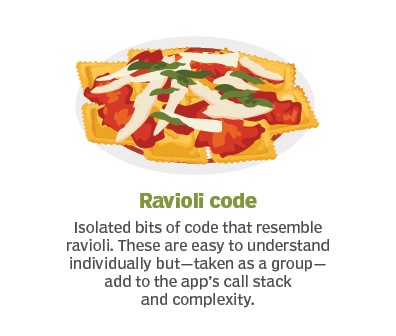
\includegraphics[scale=.5]{img/ravioli.png}
    \end{center}
\end{frame}

\begin{frame}
    \autotitle
    \begin{center}
        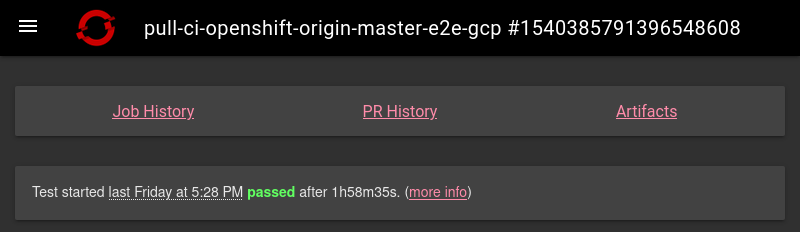
\includegraphics[width=\textwidth]{../ci-operator/img/job.png}
        \footnotesize
        \url{https://prow.ci.openshift.org/view/gs/origin-ci-test/pr-logs/pull/27275/pull-ci-openshift-origin-master-e2e-gcp/1540385791396548608}
    \end{center}
    \note{
        We will revisit today the example job we looked at in the last third of
        the previous presentation, now in much more detail.
    }
\end{frame}

\begin{frame}[fragile]
    \autotitle
    \tiny
    \url{https://gcsweb-ci.apps.ci.l2s4.p1.openshiftapps.com/gcs/origin-ci-test/pr-logs/pull/27275/pull-ci-openshift-origin-master-e2e-gcp/1540385791396548608/prowjob.json}*
    \footnotesize
    \begin{verbatim}
command:
- ci-operator
args:
- --gcs-upload-secret=/secrets/gcs/service-account.json
- --image-import-pull-secret=/etc/pull-secret/.dockerconfigjson
- --lease-server-credentials-file=/etc/boskos/credentials
- --report-credentials-file=/etc/report/credentials
- --secret-dir=/secrets/ci-pull-credentials
- --secret-dir=/usr/local/e2e-gcp-cluster-profile
- --target=e2e-gcp
    \end{verbatim}
    \vfill
    \small
    *\href{https://github.com/openshift/ci-docs/pull/266}{
        \textit{how-tos: document artifacts directory} \#266
        --- \texttt{openshift/ci-docs}
    }
    \note{
        As a reminder, this will (via \texttt{prowgen}) result in a
        \texttt{ProwJob} which will execute \texttt{ci-operator} targeting the
        single test name \texttt{e2e-gcp}, declared in its configuration file
        (obtained from the \texttt{configresolver}).
    }
\end{frame}

\begin{frame}
    \autotitle
    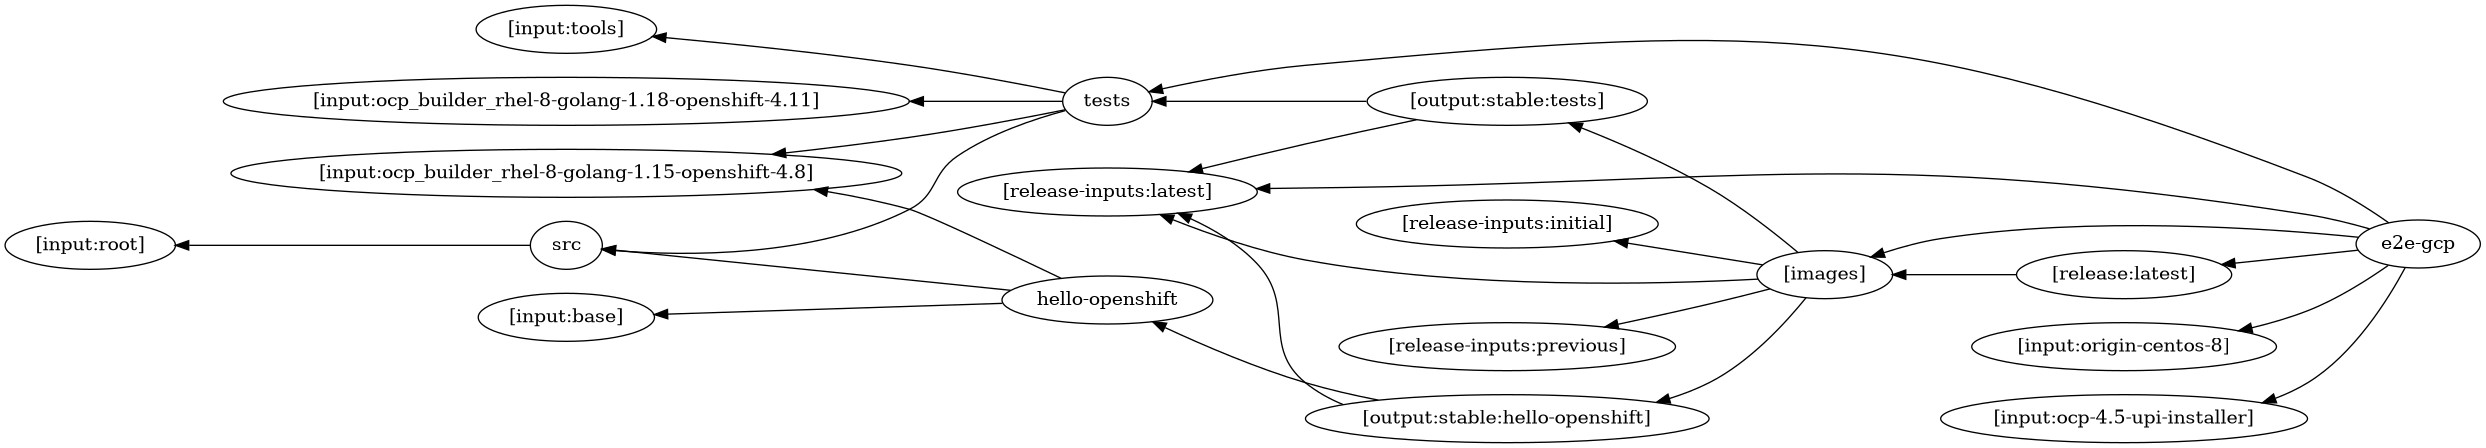
\includegraphics[width=\textwidth]{../ci-operator/img/graph_origin_gcp.jpg}
    \note{
        And this will be done by constructing and execting this step graph.  See
        the previous presentation for a reminder of how all of this generally
        works.
    }
\end{frame}

\begin{frame}[fragile]
    \autotitle
    \footnotesize
    \url{https://github.com/openshift/release/blob/master/ci-operator/config/openshift/origin/openshift-origin-master.yaml}
    \vfill
    \normalsize
    \begin{verbatim}
tests:
- as: e2e-gcp
  steps:
    cluster_profile: gcp-openshift-gce-devel-ci-2
    workflow: openshift-e2e-gcp-loki
    \end{verbatim}
    \vfill
    \note{
        It all starts with this innocent test definition in the configuration
        file\ldots
    }
\end{frame}

\section{Test definitions}
\begin{frame}
    \sectiontitleframe
\end{frame}

\begin{frame}
    \autotitle
    \begin{itemize}
        \item regular \texttt{ci-operator} test
            \begin{itemize}
                \item images
                \item release images
                \item artifacts
                \item cluster profiles
                \item \ldots
            \end{itemize}
    \end{itemize}
    \note{
        The first thing to note about multi-stage tests is that they are just
        another type of test, just as container tests are.  This
        makes all other parts of \texttt{ci-operator} easily and naturally
        available to them.

        On the implementation side, they are just another type of
        \texttt{ci-operator} step and are fully defined by the configuration
        file (and registry).  Parsing and interpreting a multi-stage test does
        not require any of the arcane techniques used in the implementation of
        template tests.
    }
\end{frame}

\begin{frame}[fragile]
    \autotitle
    \footnotesize
    \url{https://github.com/openshift/release/blob/master/ci-operator/config/openshift/ci-tools/openshift-ci-tools-master.yaml}
    \normalsize
    \begin{verbatim}
tests:
- as: e2e
  steps:
    test:
    - as: e2e
      commands: … make e2e
      from: test-bin
      # …
    \end{verbatim}
    \note{
        Multi-stage tests are defined in the configuration file just like any
        other type of test.  A multi-stage test is distinguished by the
        \texttt{steps} entry.  Definitions can be complex, but \texttt{e2e} in
        \texttt{ci-tools} is a good example of a minimal test.

        (the actual test also has a \texttt{credentials} section, which is not
        revelant for this example and will be explained later)
    }
\end{frame}

\begin{frame}[fragile]
    \autotitle
    \small
    \begin{multicols}{2}
        \begin{verbatim}
tests:
- as: e2e
  steps:
    test:
    - as: e2e
      commands: … make e2e
      from: test-bin
      # …
        \end{verbatim}
        \columnbreak
        \begin{verbatim}
tests:
- as: e2e
  commands: … make e2e
  container:
    from: test-bin
    # …
        \end{verbatim}
    \end{multicols}
    \note{
        With this format, it is equivalent to the \texttt{container} test type
        (unifying their implementation is a long-term goal).  These tests will
        have slightly different executions, but will have the same overall
        effect.
    }
\end{frame}

\subsection{Phases}

\begin{frame}
    \autotitle
    \begin{itemize}
        \item pre/test/post
        \item serial execution
            \begin{itemize}
                \item ``short-circuit'' execution for pre/test
                \item post steps always executed
            \end{itemize}
        \item each step corresponds to a \texttt{Pod}
            \begin{itemize}
                \item shared data can be placed in a special directory
            \end{itemize}
    \end{itemize}
    \note{
        What differentiates multi-stage tests from simple container tests (or
        from templates, for that matter) are the \textit{execution phases}:
        \texttt{pre}, \texttt{test}, and \texttt{post}.  Superficially, they are
        simple sequences of steps (isolated test scripts) executed in serial,
        but each phase has distinct semantic characteristics.
        \begin{description}
            \item[\texttt{pre}]
                is a sequence of preparatory steps.  It should perform the setup
                necessary for the test to be executed (e.g. creating an
                ephemeral cluster).  If any of the steps fail, it is assumed
                that the test cannot continue and the rest of the \texttt{pre}
                steps as well as all of the \texttt{test} steps are not
                executed.
            \item[\texttt{test}]
                is a sequence of one or more steps which execute the actual test
                code.  If any of the steps fail, the rest of the steps are not
                executed.
            \item[\texttt{post}]
                is a sequence of steps which releases any resources acquired by
                the previous phases.  It is always executed and, unlike the
                others, always executed in its entirety, even if some of its
                steps fail.
        \end{description}
    }
\end{frame}

\begin{frame}
    \autotitle
    \texttt{\$SHARED\_DIR}
    \begin{itemize}
        \item Small storage space for inter-step data.
        \item Implemented using a Kubernetes \texttt{Secret}.
        \item Hard 1MB limit, no directories.
        \item
            Completely rewritten by the contents of the directory in the pod
            after the step script is executed.
        \item
            State in the ephemeral cluster can be used for higher-bandwidth
            communication between steps.
        \item \texttt{kubeconfig} is treated especially.
        \item
            Data intended for debugging tests should be placed in the artifacts
            directory.
    \end{itemize}
    \note{
        Unlike template tests:

        \begin{itemize}
            \item Each step is executed in its own isolated pod.
            \item
                Execution is serial: a step is executed only after the previous
                step ends.
            \item
                \texttt{ci-operator} manages the execution of individual steps.
        \end{itemize}

        For data which has to be passed between steps, a small storage space is
        provided, which is mounted in every pod.  It is implemented using
        Kubernetes \texttt{Secret}s, so it has limitations.  However, most tests
        can use external means (such as the ephemeral OpenShift cluster) for
        larger data.  The artifacts directory is also available, just like in
        other types of tests.

        Because \texttt{ci-operator} is optimized for OpenShift E2E tests, some
        files in the shared directory (such as the \texttt{kubeconfig} for
        ephemeral clusters) are treated specially.
    }
\end{frame}

\subsection{Images}

\begin{frame}[fragile]
    \autotitle
    Images
    \begin{itemize}
        \item \texttt{from}
            \begin{itemize}
                \item pipeline images
                    \begin{itemize}
                        \item \texttt{root}, \texttt{src}, \texttt{bin}, \ldots
                        \item \texttt{base\_images}
                        \item \texttt{images}
                    \end{itemize}
                \item ``stable'' images
                    \begin{itemize}
                        \item \texttt{releases}
                        \item \texttt{tag\_specification}
                    \end{itemize}
            \end{itemize}
        \item \texttt{from\_image}
            \begin{itemize}
                \item $\approx \texttt{base\_images}$
                \item
                    \begin{verbatim}
from_image:
  namespace: ocp
  name: upi-installer
  tag: 4.12
                    \end{verbatim}
            \end{itemize}
    \end{itemize}
    \note{
        Unlike container tests, steps can be executed using any
        \texttt{ci-operator} image.  Pipeline images, which are either imported
        or built, can be used, as well as images from release streams or
        payloads.

        A mechanism (\texttt{from\_image}) exists for using imported
        images in shared test definitions.  Here, we will just note its mode of
        operation is equivalent to \texttt{base\_images}; shared definitions
        will be explained in the step registry section.
    }
\end{frame}

\subsection{Credentials}

\begin{frame}[fragile]
    \autotitle
    Credentials
    \begin{itemize}
        \item Vault $\to$ build cluster $\to$ test namespace $\to$ test pod
        \item \texttt{ci-operator} must have access to the source namespace.
        \item
            The \texttt{test-credentials} namespace is pre-configured for
            regular users.
        \item Supplanted old methods.
            \begin{itemize}
                \item \texttt{secret}
                \item \texttt{secrets}
                \item \texttt{--secret-dir}
                \item etc.
            \end{itemize}
        \item
            \begin{verbatim}
credentials:
- namespace: ns
  name: name
  mount_path: /path
            \end{verbatim}
    \end{itemize}
    \note{
        Another major improvement over other test types is the
        \texttt{credentials} section available in steps.  The \texttt{Secret}
        objects listed therein will be imported into the test namespace and
        mounted in the corresponding pods.

        The \texttt{Secret} must already exist and be accessible, but no other
        setup is necessary.  For regular users, the current flow is to create a
        secret collection in Vault and synchronize it to the build clusters
        using special values in the credentials.  A \texttt{test-credentials}
        namespace is preconfigured in each cluster for this purpose.
    }
\end{frame}

\subsection{Parameters}

\begin{frame}[fragile]
    \autotitle
    Parameters
    \begin{itemize}
        \item Key/value data declared in a step.
        \item Ultimately become environmental variables.
        \item Can be overridden (coming soon).
    \end{itemize}
    \small
    \begin{verbatim}
as: openshift-e2e-test
from: tests
commands: openshift-e2e-test-commands.sh
env:
- name: TEST_SUITE
  default: openshift/conformance/parallel
  documentation: |
    The test suite to run.  Use 'openshift-test
    run --help' to list available suites.
# …
    \end{verbatim}
    \note{
        Parameters are a way of generating slight test variations without
        needing a completely new step definition.  Ultimately, they are
        key/value data which become simple environmental variables set in the
        corresponding pods.  One or more steps can declare a parameter,
        optionally with a default value --- all parameters must be declared and
        be given a value in a test definition.

        The hierarchical relation between registry components (explained in a
        later section) allows great freedom in how parameters can be given
        values and how tests can be composed.
    }
\end{frame}

\subsection{Dependencies}

\begin{frame}[fragile]
    \autotitle
    Dependencies
    \begin{itemize}
        \item \texttt{ci-operator} image \textit{pull spec} $\to$ test pod
        \item Establishes images $\to$ test dependency.
        \item
            \begin{verbatim}
as: test-step
dependencies:
- name: pipeline:bin
  env: BIN_IMG
- name: release:4.12
  env: RELEASE_4_12\end{verbatim}
        \item
            \begin{verbatim}
#!/bin/bash
use "$BIN_IMG"
use "$RELEASE_4_12"
        \end{verbatim}
    \end{itemize}
    \note{
        Tests sometimes need to refer to imported or built images, not as their
        execution image, but as a general \textit{pull spec}.  For this, the
        \texttt{dependencies} section can be used.  \texttt{name} references
        either a pipeline or release image: the \textit{pull spec} referring to
        the image in the temporary namespace will be  available to the
        corresponding pod as an environmental variable.

        This also establishes the dependencies between the required
        (\texttt{ci-operator}) steps and the test so that the latter is only
        executed when the images are available.
    }
\end{frame}

\begin{frame}[fragile]
    \autotitle
    \small
    \begin{verbatim}
# openshift-e2e-tests-ref.yaml
dependencies:
- name: "release:latest"
  env: OPENSHIFT_UPGRADE_RELEASE_IMAGE_OVERRIDE
    \end{verbatim}
    \begin{verbatim}
# openshift-e2e-tests-commands.sh
openshift-tests run-upgrade \
    "${TEST_UPGRADE_SUITE}" \
    --to-image \
        "${OPENSHIFT_UPGRADE_RELEASE_IMAGE_OVERRIDE}" \
    --options "${TEST_UPGRADE_OPTIONS-}" \
    --provider "${TEST_PROVIDER}" \
    -o "${ARTIFACT_DIR}/e2e.log" \
    --junit-dir "${ARTIFACT_DIR}/junit"
    \end{verbatim}
    \note{
        One (simplified) example is shown here, where the upgrade test
        references whatever the \texttt{latest} release payload is in a
        particular test namespace.
    }
\end{frame}

\begin{frame}[fragile]
    \autotitle
    Leases
    \begin{itemize}
        \item \texttt{ci-operator} $\to$ Boskos $\to$ test pod
        \item Generalization of implicit lease added by cluster profiles
        \item
            Leased resource name is available to the test script via
            environmental variable.
        \item
            \begin{verbatim}
leases:
- env: OVIRT_UPGRADE_LEASED_RESOURCE
  resource_type: ovirt-upgrade-quota-slice
  count: 42
            \end{verbatim}
    \end{itemize}
    \note{
        \texttt{ci-operator} has an integration with the Boskos leasing server,
        which allows \textit{resources} of limited capacity to be declared.
        \texttt{ci-operator} will request these resources before starting the
        execution of the test, periodically renew them, and release them when
        the test ends.

        Initially (even in the template days, but also currently), this was
        triggered by cluster profiles.  Each profile is declared in
        \texttt{ci-tools} and has a resource type associated with it.

        \texttt{leases} are a generalization of this concept.  Instead of a
        cluster profile, or in addition to it, a test or registry component can
        declare additional resources which it requires before it is allowed to
        start.  The name of the resource is available as an environmental
        variable, which is often used to pass some information to the test step.
    }
\end{frame}

\subsection{etc.}

\begin{frame}
    \autotitle
    \begin{itemize}
        \item best-effort steps
        \item catalogues / optional operators
        \item \texttt{KUBECONFIG}
        \item cluster profiles
        \item \texttt{oc} CLI injection
        \item no \texttt{ServiceAccount} credentials
        \item cluster claims
        \item VPN connection
        \item \ldots
    \end{itemize}
    \note{
        This is an abbreviated list of aspects of multi-stage tests which cannot
        be covered today due to time constraints.  Contrary to template tests,
        most of the implementation is properly documented, so consult the pages
        linked at the beginning of the presentation.
    }
\end{frame}

\section{Step registry}
\begin{frame}
    \sectiontitleframe
\end{frame}

\begin{frame}
    \autotitle
    Goals
    \begin{itemize}
        \item discoverable
        \item referenceable
        \item verifiable
        \item reusable
    \end{itemize}
    \note{
        Beyond improving the implementation of tests, the design of multi-stage
        tests also had the major goal of improving the \emph{process} of
        creating tests.  It identified several attributes which the new format
        should have, discussed in the next sections.
    }
\end{frame}

\subsection{Discoverable}

\begin{frame}
    \autotitle
    \small
    \begin{itemize}
        \item \url{https://steps.ci.openshift.org}
        \item \url{https://steps.ci.openshift.org/workflow/ipi-aws}
        \item \url{https://steps.ci.openshift.org/chain/ipi-aws-pre}
        \item \url{https://steps.ci.openshift.org/reference/ipi-install-install}
    \end{itemize}
    \note{
        Each component of a test definition is easily discoverable.  There is no
        longer the need to excavate giant \texttt{bash} scripts embedded in YAML
        definitions.  \texttt{steps.ci.openshift.org} is a web interface for
        test definitions which is heavily cross-linked.  All jobs, tests, and
        registry components are listed, in a manner which makes it easy to
        discover exactly how a test is or can be defined.
    }
\end{frame}

\subsection{Referenceable}

\begin{frame}[fragile]
    \autotitle
    \footnotesize
    \url{https://prow.ci.openshift.org/view/gs/origin-ci-test/logs/periodic-ci-openshift-release-master-okd-4.10-e2e-vsphere/1579723667426775040}
    \vspace{\baselineskip}
    \begin{verbatim}
Running step e2e-vsphere-ipi-install-install.
Logs for container test in pod e2e-vsphere-ipi-install-install:
…
Step e2e-vsphere-ipi-install-install failed after 23m20s.
Step phase pre failed after 40m10s.
…
Link to step on registry info site: …
Link to job on registry info site: …
    \end{verbatim}
    \note{
        When a job fails, the \texttt{ci-operator} output includes links to the
        definitions of the steps which failed.
    }
\end{frame}

\begin{frame}
    \autotitle
    \footnotesize
    \url{https://steps.ci.openshift.org/workflow/ipi-aws\#approvers}
    \normalsize
    \begin{itemize}
        \item wking
        \item vrutkovs
        \item abhinavdahiya
        \item deads2k
        \item staebler
        \item technical-release-team-approvers
        \item jianlinliu
        \item yunjiang29
    \end{itemize}
    \note{
        Each of those pages also has links to the definition in GitHub, as well
        as a list of its \texttt{OWNERS} (reviewers and approvers).  This way,
        the error output has (in principle) the information required to go from
        a failure to the possible cause and to those who may be able to assist.
    }
\end{frame}

\subsection{Verifiable}

\begin{frame}[fragile]
    \autotitle
    \footnotesize
    \begin{itemize}
        \item \texttt{pull-ci-openshift-release-master-step-registry-shellcheck}
        \item \url{https://www.shellcheck.net}
        \item
            \begin{verbatim}
find ci-operator/step-registry -name '*.sh' -print0 \
    | xargs -0 -n1 shellcheck -S warning
            \end{verbatim}
    \end{itemize}
    \note{
        The quality of scripts in the step registry is verified using
        \texttt{shellcheck}, a (Haskell) program which identifies problems in
        \texttt{bash} source code (syntax errors, unquoted variables, etc.).  It
        is executed as a blocking pre-submit job which verifies every shell
        script in the registry directory.
    }
\end{frame}

\subsection{Reusable}

\begin{frame}
    \autotitle
    \begin{itemize}
        \item reference
        \item chain
        \item workflow
    \end{itemize}
    \note{
        The step registry is a central place where parts of test definitions are
        stored.  Several types of registry \textit{components} can be combined
        and used by a large number of tests.
    }
\end{frame}

\begin{frame}[fragile]
    \autotitle
    \footnotesize
    \url{https://steps.ci.openshift.org/reference/ipi-install-install}
    \vspace{\baselineskip}
    \begin{verbatim}
ref:
  as: ipi-install-install
  from: installer
  grace_period: 10m
  commands: ipi-install-install-commands.sh
  cli: latest
  resources:
    requests:
      cpu: 1000m
      memory: 2Gi
    \end{verbatim}
    (cont.)
    \note{
        A \textit{reference} is the lowest level of step definition.  It
        corresponds directly to the step definition inline in a test shown in
        previous examples.  In this way, sharing code between tests can be as
        simple as moving a step definition virtually unchanged to the registry
        and referencing it.

        In this example, the installation step which creates ephemeral clusters
        is defined once in the registry and used everywhere it is needed with a
        simple \texttt{ref: ipi-install-install}.
    }
\end{frame}

\begin{frame}[fragile]
    \autotitle
    \footnotesize
    (cont.)
    \begin{verbatim}
  credentials:
  - namespace: test-credentials
    name: loki-stage-collector-test-secret
    mount_path: /var/run/loki-secret
  # …
  env:
  - name: OPENSHIFT_INSTALL_EXPERIMENTAL_DUAL_STACK
    default: "false"
    documentation: Using experimental Azure dual-stack support
  # …
  dependencies:
  - name: "release:latest"
    env: OPENSHIFT_INSTALL_RELEASE_IMAGE_OVERRIDE
  # …
  documentation: |-
    The IPI install step runs the OpenShift Installer …
    \end{verbatim}
\end{frame}

\begin{frame}[fragile]
    \autotitle
    \footnotesize
    \url{https://steps.ci.openshift.org/chain/ipi-aws-pre}
    \vspace{\baselineskip}
    \begin{verbatim}
chain:
  as: ipi-aws-pre
  steps:
  - chain: ipi-conf-aws
  - chain: ipi-install
  documentation: |-
    The IPI setup step contains all steps that provision an
    OpenShift cluster with a default configuration on AWS.
    \end{verbatim}
    \note{
        Sequences of steps can be combined into \textit{chains}, which are
        analogous to the phases of a multi-stage test.  Chains are the main
        method of code reuse in the registry.  Beyond simply grouping steps,
        they can also contain definitions for step parameters and other options,
        as explained later.
    }
\end{frame}

\begin{frame}[fragile]
    \autotitle
    \footnotesize
    \url{https://steps.ci.openshift.org/workflow/ipi-aws}
    \vspace{\baselineskip}
    \begin{verbatim}
workflow:
  as: ipi-aws
  steps:
    pre:
    - chain: ipi-aws-pre
    post:
    - chain: ipi-aws-post
  documentation: |-
    The IPI workflow provides pre- and post- steps that
    provision and deprovision an OpenShift cluster with a
    default configuration on AWS, allowing job authors to
    inject their own end-to-end test logic.

    All modifications to this workflow should be done by
    modifying the `ipi-aws-{pre,post}` chains to allow other
    workflows to mimic and extend this base workflow without
    a need to backport changes.
    \end{verbatim}
    \note{
        Finally, a complete test definition can be grouped into a
        \textit{workflow}.  A workflow definition is exactly the same as a test
        definition, and usually encapsulates a test flow from beginning to end.

        With a workflow, a shared test definition can be as simple as a few
        lines.  If necessary, each phase (i.e. \texttt{pre}, \texttt{test},
        \texttt{post}) can still be redefined in the test which includes the
        workflow.  This will replace the entire sequence of steps for that
        particular phase.
    }
\end{frame}

\begin{frame}[fragile]
    \autotitle
    \begin{multicols}{2}
        \begin{verbatim}
as: e2e-aws
steps:
  pre:
  - as: conf-this
    commands: # …
  - as: conf-that
    commands: # …
  - as: install
    commands: # …
  - as: rbacs
    commands: # …
        \end{verbatim}
        \columnbreak
        \begin{verbatim}
  test:
  - as: test
    commands: # …
  post:
  - as: gather-this
    commands: # …
  - as: gather-that
    commands: # …
  - as: uninstall
    commands: # …
        \end{verbatim}
    \end{multicols}
    \note{
        The next few examples will demonstrate the process of going from a
        completely idiosyncratic test to one that can be shared by multiple
        definitions in a few lines of YAML.

        This definition shows a typical OpenShift E2E test: a cluster is created
        based on some configuration steps, the tests are executed, and the
        cluster is destroyed.  Here, \texttt{commands\ldots} in each definition
        stands for the particular entries which would be declared in each step,
        which can anywhere from several lines to several pages long.
    }
\end{frame}

\begin{frame}[fragile]
    \autotitle
    \begin{multicols}{2}
        \begin{verbatim}
as: e2e-aws
steps:
  pre:
  - ref: conf-this
  - ref: conf-that
  - ref: install
  - ref: rbacs
  # …
        \end{verbatim}
        \columnbreak
        \begin{verbatim}
ref:
  as: conf-this
  commands: # …
        \end{verbatim}
        \begin{verbatim}
ref:
  as: conf-that
  commands: # …
        \end{verbatim}
        \ldots
    \end{multicols}
    \note{
        The first\ldots{} step in the process would be to move individual step
        definitions to the registry and replace the original ones with
        references.  This allows any number of tests to use the shared
        definition and is already an enormous improvement over template tests.
    }
\end{frame}

\begin{frame}[fragile]
    \autotitle
    \begin{multicols}{2}
        \begin{verbatim}
as: e2e-aws
steps:
  pre:
  - chain: aws-pre
  test: # …
  post:
  - chain: aws-post
        \end{verbatim}
        \columnbreak
        \begin{verbatim}
chain:
as: aws-pre
  steps:
  - ref: conf-this
  - ref: conf-that
  - ref: install
  - ref: rbacs
        \end{verbatim}
        \begin{verbatim}
chain:
as: aws-post
steps:
# …
        \end{verbatim}
    \end{multicols}
    \note{
        Next, a sequence of steps from the registry can be placed in one or more
        chains.  This allows the sequence (and/or its configuration) to be
        changed without the need to modify every test definition.
    }
\end{frame}

\begin{frame}[fragile]
    \autotitle
    \begin{multicols}{2}
        \begin{verbatim}
as: e2e-aws
steps:
  workflow: aws-ipi
  test: # …
        \end{verbatim}
        \columnbreak
        \begin{verbatim}
workflow:
  as: aws-ipi
  pre:
  - chain: aws-pre
  post:
  - chain: aws-post
        \end{verbatim}
    \end{multicols}
    \note{
        A complete test pattern (e.g. ``E2E test on AWS'') can then be put into
        a workflow.  This abstracts the setup and cleanup phases so that the
        test definition contains only a reference to the workflow and the actual
        test steps which are to be executed.
    }
\end{frame}

\begin{frame}[fragile]
    \autotitle
    \begin{columns}[t]
        \column{0.4\textwidth}
        \begin{verbatim}
as: e2e-aws
steps:
  workflow: aws-ipi
        \end{verbatim}
        \column{0.55\textwidth}
        \begin{verbatim}
workflow:
  as: openshift-e2e-aws
  pre:
  - chain: aws-pre
  test:
  - ref: openshift-e2e-test
  post:
  - chain: aws-post
        \end{verbatim}
    \end{columns}
    \note{
        Going even further, an entire test suite can be shared among several
        repositories.  In this case, the ``OpenShift on AWS E2E'' test suite is
        put into its own workflow (n.b.: which shares the pre/post chains with
        other workflows).  Repositories can include this entire suite by simply
        declaring a test which references the workflow.
    }
\end{frame}

\begin{frame}[fragile]
    \autotitle
    \footnotesize
    \begin{verbatim}
$ find ci-operator/step-registry/ -name 'ipi-conf-*-ref.yaml' \
    | wc -l
75
$ find ci-operator/step-registry/ -name 'ipi-conf-*-ref.yaml' \
    | sed 's,.*/,,; s/-ref\.yaml//' | shuf | head -15 | sort
ipi-conf-additional-enabled-capabilities
ipi-conf-alibabacloud
ipi-conf-azure-provisioned-des
ipi-conf-azurestack-creds
ipi-conf-azure-vmgenv1
ipi-conf-azure-workers-marketimage
ipi-conf-etcd-on-ramfs
ipi-conf-libvirt
ipi-conf-openstack-enable-octavia
ipi-conf-ovirt-generate-csi-test-manifest
ipi-conf-ovirt-generate-csi-test-manifest-release-4.6-4.8
ipi-conf-ovirt-generate-install-config
ipi-conf-ovirt-generate-install-config-params
ipi-conf-ovirt-generate-ovirt-config
ipi-conf-vsphere-zones
    \end{verbatim}
    \note{
        Since the configuration and installation steps have their own chains in
        the registry, it is very easy to combine one or more configuration steps
        to create a specific test scenario, then include all of the other
        registry components which implement the machinery behind the test
        (cluster installation, artifact gathering, etc.).

        A quick look at the registry shows there is a large number of
        configuration steps, many of which can be combined (e.g. to create a
        test on a cluster with "additional capabilities" and "\texttt{etcd} on
        \texttt{ramfs} using \texttt{libvirt}).
    }
\end{frame}

\begin{frame}[fragile]
    \autotitle
    \footnotesize
    \url{https://docs.ci.openshift.org/docs/architecture/step-registry/#hierarchical-propagation}
    \vspace{\baselineskip}
    \normalsize
    \begin{verbatim}
as: openshift-e2e-test
env:
- name: TEST_SUITE
# …
    \end{verbatim}
    \note{
        One last, more advanced method of reuse is what is called
        \textit{hierarchical propagation}.  Registry components used by a test
        are arranged as a tree: the test can include a workflow, which can
        include any number of chains, which can themselves include chains
        recursively, which ultimately include steps.

        When all of these definitions are assembled to generate the final step
        list executed by the test, several configuration options are propagated
        from the root of the tree to the leaves (namely: parameters,
        dependencies, leases).  This means definitions in tests override those
        in workflows, which in turn override those in chains, which in turn
        override those in steps.  These definitions are strictly checked such
        that every option declared in a parent component has to be declared in a
        subcomponent and has to have a resulting value after this process
        completes.
    }
\end{frame}

\begin{frame}[fragile]
    \autotitle
    \begin{verbatim}
tests:
- as: e2e
  steps:
    test:
    - ref: openshift-e2e-test
    env:
      TEST_SUITE: openshift/conformance/parallel
    \end{verbatim}
    \note{
        In this example, a test includes the step shown in the previous slide
        and specifies a value for its parameter.  It must do so, since the
        parameter does not have a default.  Similarly, giving the parameter a
        value without including a step which declares it would be an error.
    }
\end{frame}

\begin{frame}[fragile]
    \autotitle
    \begin{verbatim}
workflow:
  as: openshift-e2e-serial
  steps:
    test:
    - ref: openshift-e2e-test
    env:
      TEST_SUITE: openshift/conformance/serial
    \end{verbatim}
    \begin{verbatim}
tests:
- as: e2e
  steps:
    workflow: openshift-e2e-serial
    \end{verbatim}
    \note{
        Hierarchical propagation allows the parameter value to be defined in a
        workflow (or a chain).  This way, any test which includes the workflow
        will use that value for the parameter, since it would propagate down
        from the workflow to the step.

        While nonsensical in this case, the test could also give the parameter a
        value, which would override the value in the workflow, since tests are
        the root of the resolution tree.
    }
\end{frame}


\begin{frame}
    \usebeamertemplate{end page}
\end{frame}

\end{document}
